\documentclass[a4paper,12pt]{article}

%%% Поля
\usepackage[
    left=2cm,
    right=2cm,
    top=2cm,
    bottom=3cm,
    bindingoffset=0cm
]{geometry}

%%% Работа с русским языком
\usepackage{cmap}                       % поиск в PDF
\usepackage{mathtext}                   % русские буквы в формулах
\usepackage[T2A]{fontenc}               % кодировка
\usepackage[utf8]{inputenc}             % кодировка исходного текста
\usepackage[english,russian]{babel}     % локализация и переносы
\usepackage{indentfirst}
\frenchspacing

%%% Дополнительная работа с математикой
\usepackage{amsmath,amsfonts,amssymb,amsthm,mathtools}  % AMS

%%% Текст в колонки
\usepackage{multicol}

%%% Списки
\usepackage{enumitem}
\setlist{nosep, leftmargin=*}
\renewcommand{\labelenumi}{\arabic*)}

%%% Системы уравнений
\usepackage{cases}

%%% Таблицы
\usepackage{array}
\usepackage{makecell}

%%% Рисунки
\usepackage{graphicx}
\usepackage{float}

%%% Точка в подписях к рисункам
\usepackage[labelsep=period]{caption}

%%% Список литературы
\usepackage[
    natbib = true,
    style = alphabetic,
    sorting = none,
    backend = biber,
    language = autobib,
    autolang = other
]{biblatex}
\addbibresource{references.bib}

%%% Исправление символа номера при использовании gost-numeric.bbx
\usepackage{textcomp}
\DefineBibliographyStrings{russian}{number={\textnumero}}

%%% Гиперссылки
\usepackage[pdftex,unicode]{hyperref}

%%% Перенос знаков в формулах (по Львовскому)
\newcommand*{\hm}[1]{#1\nobreak\discretionary{}{\hbox{$\mathsurround=0pt #1$}}{}}


%%% Свои команды

\newcommand{\forcehyphenation}{-\linebreak}

\newcommand{\absent}[1]{[...#1...]}


%%% Свои операторы
\DeclareMathOperator*{\argmin}{{argmin}}
\DeclareMathOperator*{\argmax}{{argmax}}


%%% Заглавие
\title{Классификация русских классических стихов \\ по эпохам}
\author{Пономарев Андрей Сергеевич}
\date{2024--2025 учебный год, \\ весенний семестр}


\begin{document}
\maketitle

\begin{abstract}
    \absent{Краткое описание проекта} Репозиторий проекта находится по ссылке \\
    \url{https://github.com/ponomarevandr/russian_poems_classification}.
\end{abstract}



\section{Введение}

Обработка естественного языка (natural language processing)~-- область информатики, в настоящее время переживающая бурное развитие. Ее методы находят широкое применение в самых разных прикладных задачах. Из-за подобной широты многие задачи все еще далеки от исчерпывающего анализа, существующие решения можно свободно дорабатывать и развивать.

Одним из разделов обработки естественного языка, которые поныне не находятся в центре внимания, является анализ стихотворных текстов. Об этом свидетельствует как относительно малое число публикаций по теме, так и слова их авторов напрямую (например, \cite{barbado2021}).

В настоящем проекте предлагается решение задачи классификации русских классических стихотворений по эпохе, или, иначе, течению, направлению. Автор не нашел в Интернете статей, освещавших бы в точности этот вопрос, и в этом смысле работа нова.

Будут рассмотрены два подхода к решению задачи: с помощью нейронной сети LSTM (в качестве базового) и с помощью предобученной модели RuBERT-tiny.

Лучший результат показала модель RuBERT-tiny~-- точность около $70 \%$. Она в дальнейшем может применяться на практике, например, для категоризации стихотворений в Интернете, как классических, так и современных.


\subsection{Команда}

Проект подготовил \textbf{Пономарев А. С.}


\section{Смежные работы}

Перечислим несколько статей, близких проекту по тематике.

Работа \cite{noraini2012} посвящена классификации малайской поэзии по нескольким темам. Статья написана давно и использует ныне устаревший подход~-- метод опорных векторов (SVM) поверх TF-IDF,~-- но подходит для знакомства с задачей.

Интересна и обширна статья \cite{ruma2022}. Авторы рассматривают задачу классификации стихотворений Хафиза Ширази (на персидском языке) по периодам в жизни автора, что совсем близко к теме настоящего проекта. Основная используемая модель~-- LSTM-нейросеть, но помимо нее авторы пробуют логистическую регрессию, SVM, random forest, Bi-LSTM, GRU; в качестве эмбеддингов~-- CBOW, SkipGram, а также их конкатенацию. Авторы утверждают, что добились внушительной точности в $85 \%$.

Отметим также близкую по тематике работу \cite{orabi2020}, посвященную классификации арабской поэзии по эпохе написания. Авторы используют CNN-нейросеть с эмбеддингами FastText, относительно большой датасет (десятки тысяч стихотворений) и получают точность порядка $80 \%$.

В работе \cite{barbado2021} исследуется применение моделей-трансформеров для разбиения испанских сонетов по категориям выражаемых чувств. Для различных классов авторы добиваются F1-метрики от $0.6$ до $0.8$.

В отдельную ветвь можно выделить исследования, приспосабливающие для анализа стихотворных текстов предобученные BERT-подобные модели. В работе \cite{shahriar2023} дообучена модель AraBERT для классификации арабской поэзии по выражаемым эмоциям (точность $76.5 \%$). Статья \cite{rosa2023} описывает масштабный труд по обучению модели ALBERTI~-- мультиязыкового кодировщика для анализа стихотворений~-- на огромном массиве данных в миллионы произведений. Авторы утверждают, что на момент создания как сама модель, так и показанные результаты не имели аналогов. В работе также затронута интересная тема анализа средствами машинного обучения метрики стиха (то есть рисунка слогов и ударений).


\section{Данные}

Для работы с моделями был создан и размечен датасет русских классических стихов. За основу взяты два ранее существовавших датасета стихов, размещенные в открытом доступе: \cite{russian_poetry_corpus} и \cite{russian_poems_19000}.

После объединения исходных датасетов данные были приведены к единому формату и очищены (см. Юпитер-тетрадку \textit{dataset\_preparation.ipynb}). Итоговая структура датасета показана в таблице \ref{tab:dataset}.

Поле \textit{author} всюду приведено к одной лишь фамилии автора; в случае совпадений используются приписки через дефис, например: \textit{Багрицкий-отец}, \textit{Иванов-В}. Исключены иноязычные авторы, представленные в переводах.

Заглавие в поле \textit{title} приведено к нижнему регистру и очищено ото всех небуквенных символов, кроме цифр и пробелов.

\begin{table}[t]
\centering
\begin{tabular}[t]{|m{1.4cm}|m{2.8cm}|m{4.2cm}|m{2.9cm}|m{1.3cm}|m{1.4cm}|}
    \hline
    & \textbf{author} & \textbf{epoch} & \textbf{title} & \textbf{part} & \textbf{text} \\
    \hline
    \hline
    Содер\-жание & \makecell[l]{Фамилия \\ автора} \par & \makecell[l]{Эпоха (течение, \\ направление)} \par & Заглавие & Номер фрагмента & Текст фрагмента \\
    \hline
    Формат & Русские буквы: заглавная, далее строчные; дефис & \makecell[l]{Одно из: \\ классицизм, \\ золотой век, \\ критический реализм, \\ серебряный век, \\ футуризм, \\ соцреализм, \\ шестидесятники} \par & Строчные русские и~английские буквы, цифры, пробел & Индекс с нуля & $8$--$40$ строк, без пустых строк \\
    \hline
\end{tabular}
\caption{Структура датасета.}
\label{tab:dataset}
\end{table}

В текстах стихотворений по возможности исправлены ошибочные символы, удалены теги, сноски, номера строф, символьные артефакты. Убраны пустые строки. Исключены записи, состоящие преимущественно не из русских букв или имеющие среднюю длину строки более $60$ символов.

Из датасета удалены дубликаты. Их поиск велся как по заглавию, так и по расстоянию Левенштейна между текстами.

При работе с моделью было решено использовать стихотворные тексты длиной от $8$ до $40$ строк включительно. Для этого все более длинные произведения были <<нарезаны>> на фрагменты допустимой случайной длины. Эмпирически установлено, что распределение длин коротких стихотворений в строках близко к гамма-распределению, $\xi \sim \text{Gamma}[\alpha, \beta]$, с матожиданием $\text{E} \xi \approx 18.23$ и дисперсией $\text{D} \xi \approx 81.66$. Напомним, что его плотность определяется формулой
\[
    p_{\alpha, \beta}(x) = \cfrac{\beta^\alpha x^{\alpha - 1} e^{-\beta x}}{\Gamma(\alpha)},
\]
а также верно $\text{E} \xi = \alpha / \beta$ и $\text{D} \xi = \alpha / \beta^2$. Случайные длины при разбиении стихотворений на фрагменты получались округлением элементов выборки из описанного распределения.

Поле \textit{epoch} является целевым признаком. Будем называть его эпохой стихотворения (синонимы~-- течение, направление). Выделим семь основных эпох: см. таблицу \ref{tab:epoches}. Каждая эпоха имеет своеобразные черты и примерную датировку, представление о которых дают многочисленные открытые источники. Однако автору неизвестно единого исследования, которое давало бы исчерпывающее и достаточно строгое разбиение русской поэзии по эпохам, поэтому он в немалой степени руководствовался личной интуицией и чувством прекрасного.

\begin{table}[t]
\centering
\begin{tabular}[t]{|m{3.4cm}|m{3.6cm}|m{8cm}|}
    \hline
    Эпоха & \makecell[l]{Примерная \\ датировка} & Комментарий \\
    \hline
    \hline
    Классицизм & XVIII век & \\
    \hline
    \makecell[l]{Золотой век \\ русской поэзии} & Первая половина XIX века & \\
    \hline
    \makecell[l]{Критический \\ реализм} & Вторая половина XIX века & Близко к понятию <<натуральной школы>> \\
    \hline
    \makecell[l]{Серебряный век \\ русской поэзии} & Начало XX века & Близко к понятию символизма \\
    \hline
    Футуризм & Начало XX века & Может рассматриваться как часть Серебряного века, но резко выделяется и достаточно объемен \\
    \hline
    Социалистический реализм & Середина XX века & \\
    \hline
    \makecell[l]{Поэзия \\ шестидесятников} & Вторая половина XX века & \\
    \hline
\end{tabular}
\caption{Эпохи, выделяемые в русской поэзии}
\label{tab:epoches}
\end{table}

Для простоты будем считать, что эпоха стихотворения определяется эпохой его автора; $189$ авторам, представленным в датасете, были присвоены метки в соответствии со сказанным выше, а затем перенесены на соответствующие фрагменты произведений. Списки авторов по эпохам см. в Юпитер-тетрадке \textit{dataset\_labeling.ipynb}.

Получившееся разбиение на классы относительно сбалансированно: самый большой~-- Серебряный век~-- содержит $16204$ стихотворных фрагмента; самый малый~-- шестидесятники~-- $3238$, что примерно в $5$ раз меньше.

Для работы с моделями датасет разбивался на три части: тренировочную (train), валидационную (eval) и тестовую (test)~-- в соотношении $70:15:15$.


\section{Модели}

\subsection{LSTM}

Первая использованная модель, и она же взятая в качестве базового решения (base\-line),~-- это нейронная сеть типа Long short-term memory (LSTM) (см. Юпитер-тетрадку \textit{training\_lstm.ipynb}). Для работы выбрана известная реализация из библиотеки Pytorch~-- класс \textit{nn.LSTM}. Поверх стандартной LSTM-нейросети добавлен полносвязный линейный слой (\textit{nn.Linear}) с функцией активации LogSoftmax для получения логарифмированных вероятностей классов.

Для кодирования текста используются готовые русскоязычные эмбеддинги \textit{word2vec-ruscorpora-300} из библиотеки Gensim. Для их работы требуется лемматизация и определение части речи; то и другое производится средствами библиотеки Pymorphy3 пословно.

Нейросеть \textit{nn.LSTM} имеет размерность входа $300$, размерность внутреннего состояния $400$ и единственный скрытый слой.

Для обучения использовался оптимизатор \textit{optim.Adam} с параметром $lr = 1.5 \cdot 10^{-4}$ (learning rate).

\subsection{RuBERT-tiny}

Вторая использованная модель -- это BERT-подобный кодировщик RuBERT-tiny2 (см. Юпитер-тетрадку \textit{training\_rubert.ipynb}), опубликованный в Интернете \cite{rubert_model}. Модель была выбрана, во-первых, потому, что специально предназначена для русскоязычных текстов, во-вторых, из-за своего сравнительно малого (как и обещеат название) размера в $29.4$ миллиона параметров.

Работа с моделью происходит через библиотеки Datasets, Evaluate и Transformers компании Hugging Face. Автор значительно опирался на код из Юпитер-тетрадки \cite{rubert_notebook}. Хотя исходно модель RuBERT-tiny2 -- это кодировщик, а не классификатор, средства библиотек позволяют загрузить ее в класс \textit{AutoModelForSequenceClassification}, автоматически добавляя необходимые элементы. Для обучения использовался оптимизатор \textit{optim.Adam} из библиотеки Pytorch, с параметром $lr = 10^{-5}$. Модель поддерживает работу на GPU (Cuda), что значительно ускорило обучение -- средствами Google Colab оно было завершено приблизительно за 25 минут.

\begin{figure}[!tbh]
    \centering
    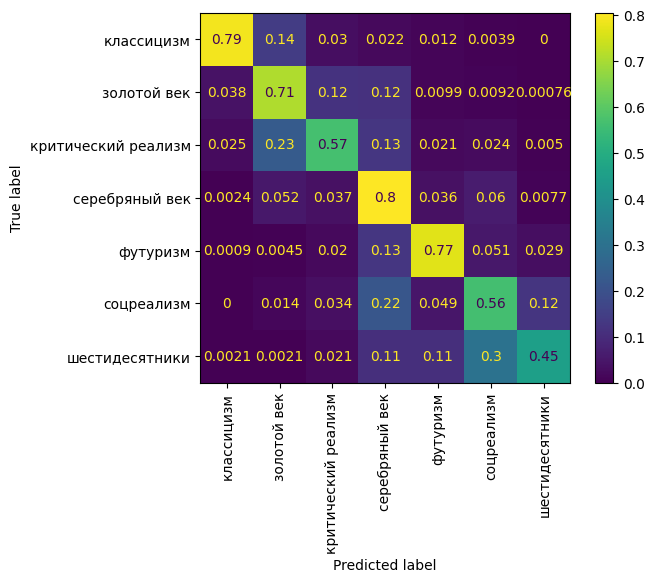
\includegraphics[width=0.7\linewidth]{figures/rubert_confusion_matrix.png}
    \caption{Матрица конфуза модели RuBERT}
    \label{fig:rubert_confusion}
\end{figure}

\section{Experiments}
This section should include several subsections.
\subsection{Metrics}
First of all, you should describe the metric(s) you were using to evaluate your approach. Most likely a metric description will include a formula.

\subsection{Experiment Setup}
Secondly, you need to describe the design of your experiment, e.g. how many runs there were, how the data split was done. The important details of your model, like hyper-parameters used in the experiments, and so on.

\subsection{Baselines}
Another important feature is that you could provide here the description of some simple approaches for your problem, like logistic regression over TF-IDF embedding for text classification. The baselines are needed is there is no previous art on the problem you are presenting.

\section{Results}
In this section, you need to list and describe the achieved results. It is crucial to have the results of the experiments for the other approaches. This is needed to be able to compare your results with some competitors. Most preferably, you should provide some references with results on the same problem.

Almost inevitably the results are presented as a table, but it is also possible to have a graph, i.e. a figure.

You need also to provide an interpretation of the presented results, to describe some features. E.g. your approach shows higher results on the short texts or by one metric instead of another.

Also in this section, you could provide some results for your model inference. The samples could be found in Tab.~\ref{tab:output}.

\begin{table}[!tbh]
    \centering
    \begin{tabular}{|c|}
\hline
Это пример вывода вашей модели на русском.\\
This is a sample output of your model in English.
\\
\hline
    \end{tabular}
    \caption{Output samples.}
    \label{tab:output}
\end{table}

\section{Conclusion}
In this section, you need to describe all the work in short: what you have done and what has been achieved. E.g. you have collected a dataset, made a markup for it and developed a model showing the best results compared to other models. 


\begin{otherlanguage}{english}
\printbibliography[
    heading=bibintoc
]
\end{otherlanguage}

\end{document}